%% CIELAB color space
%% Vilson Vieira <vilson@void.cc> - http://automata.cc - 2013 - copyleft

\documentclass{minimal}
\usepackage{tikz}

\begin{document}
  
  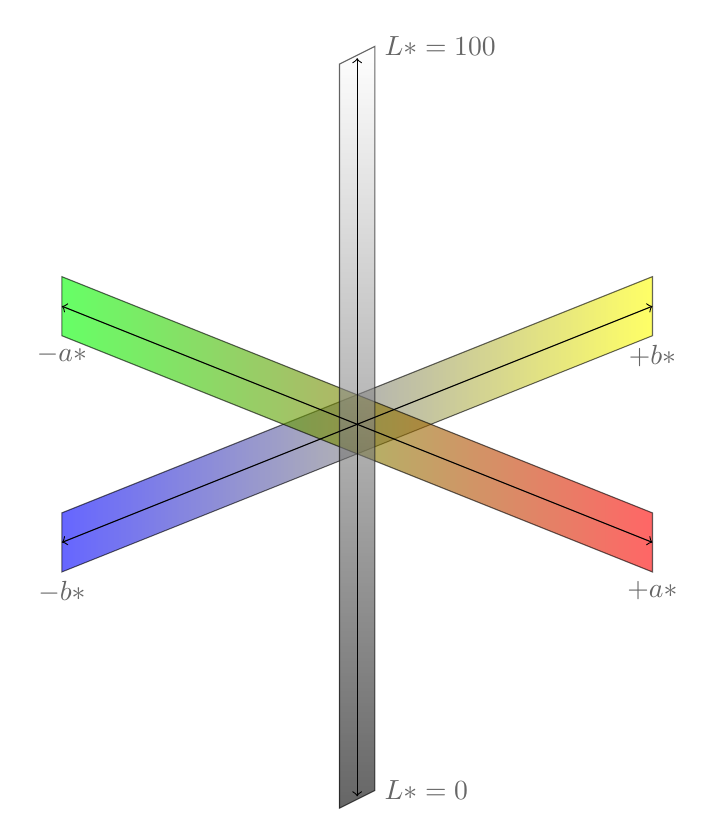
\begin{tikzpicture}[scale=1.5]
    % b* shade
    \path[draw, shade, left color=blue, right color=yellow, opacity=.6] 
    (0,0,0) node[below] {$-b*$} -- (5,2.0,0) node[below] {$+b*$} -- (5, 2.5, 0)
    -- (0, 0.5, 0) -- cycle;

    % a* shade
    \path[draw, shade, left color=green, right color=red, opacity=.6] 
    (0, 2.0, 0) node[below] {$-a*$} -- (5, 0, 0) node[below] {$+a*$} 
    -- (5, .5, 0) -- (0, 2.5, 0) -- cycle;
    
    % L* shade
    \path[draw, shade, top color=white, bottom color=black, opacity=.6] 
    (2.65, -1.85, 0) node[right] {$L* = 0$} -- (2.65, 4.45, 0) node[right] {$L*=100$}
    -- (2.35, 4.3, 0)  -- (2.35, -2., 0) -- cycle;

    % b*-axis
    \draw[<->] (0,0.25,0) -- (5, 2.25, 0);
    % a*-axis
    \draw[<->] (0,2.25,0) -- (5, 0.25, 0);
    % L*-axis
    \draw[<->] (2.5,-1.90,0) -- (2.5,4.35,0);

  \end{tikzpicture}
\end{document}
